\chapter{Dinámica relativista}\label{ch:b3:relativistic-dynamics}

En 1964, William Bertozzi filmó electrones lanzados por un acelerador
lineal: a cada paquete se le daba una energía medida y se cronometraba su
velocidad a lo largo de \qty{8.4}{m} de vuelo. Newton predecía que unos
electrones de \qty{15}{MeV} debían volar a ocho veces la velocidad de la luz;
el cronómetro dijo $0.9999c$ y se negó a ir más allá por mucho que se
empujara a los electrones. La cinemática nos dijo en el capítulo anterior
que $c$ es un límite; la dinámica debe explicar ahora qué le ocurre al
empuje --- adónde va el trabajo cuando la velocidad ya no crece. La
respuesta reorganiza la mecánica en torno a un momento nuevo y a una energía
nueva, unidos en la ecuación más famosa de la física: la energía almacenada
es masa y la masa es energía residente, $E = mc^2$. Este capítulo construye
esa dinámica y la pone luego a trabajar allí donde vive a diario ---
desintegraciones radiactivas, colisiones de partículas y los aceleradores
que convierten movimiento en materia nueva.

\section{El momento y la energía, reconstruidos}

\begin{remark}[Por qué hubo que jubilar a $m\vect v$]\label{rem:b3:relativistic-dynamics:why}
El momento clásico $m\vect v$ se conserva en todo sistema \emph{si} las
velocidades se transforman à la Galileo. No lo hacen
(\cref{prop:b3:relativistic-kinematics:addition}): una colisión que
conserva $\sum m\vect v$ en un sistema deja de hacerlo en otro, de modo que
el momento antiguo no puede ser una ley de la naturaleza --- a lo sumo la
sombra de una a baja velocidad. El arreglo consiste en medir la velocidad
con el reloj \emph{propio} de la partícula: $\dd\vect r/\dd\tau =
\gamma\,\vect v$ se transforma limpiamente, y $m\,\dd\vect r/\dd\tau$
resulta conservarse en todos los sistemas a la vez.
\end{remark}

\begin{definition}[Momento y energía relativistas]\label{def:b3:relativistic-dynamics:momentum-energy}
\index{momento relativista}\index{energía relativista}\index{energía en reposo}
Una partícula de masa $m$ y velocidad $\vect v$ ($\gamma = 1/\sqrt{1 -
v^2/c^2}$) lleva el momento y la energía
\[
\vect p = \gamma m\vect v , \qquad
E = \gamma mc^2 .
\]
En reposo, $E_0 = mc^2$: la \emph{energía en reposo}. La energía cinética es
lo que añade el movimiento, $E_k = E - mc^2 = (\gamma - 1)mc^2$, que para $v
\ll c$ se reduce al conocido $\tfrac12 mv^2$ (desarróllese $\gamma$). En todo
proceso aislado se conservan el $\vect p$ total y la $E$ total --- energías
en reposo incluidas.
\end{definition}

\begin{theorem}[La relación energía--momento]\label{thm:b3:relativistic-dynamics:relation}
\index{relación energía--momento}
Para toda partícula,
\[
E^2 = (pc)^2 + (mc^2)^2 ,
\qquad
\vect v = \frac{\vect p\,c^2}{E} :
\]
la combinación $E^2 - p^2c^2 = m^2c^4$ tiene el mismo valor en todo sistema
--- es a la energía y al momento lo que el intervalo es al tiempo y al
espacio. Dos regímenes: a baja velocidad, $E \approx mc^2 + p^2/2m$; a alta
energía ($E \gg mc^2$), $E \approx pc$ y $v \to c$: empujar más fuerte añade
energía y momento, y casi nada de velocidad.
\end{theorem}

\begin{proof}
$E^2 - p^2c^2 = \gamma^2m^2c^4(1 - v^2/c^2) = m^2c^4$; y $pc^2/E =
\gamma mvc^2/\gamma mc^2 = v$. La invariancia se sigue de que $m$
y $c$ no dependen del sistema.
\end{proof}

\begin{proposition}[Partículas sin masa]\label{prop:b3:relativistic-dynamics:massless}
\index{fotón!momento}
Una partícula de masa nula cumple $E = pc$ y se mueve exactamente a $c$ en
todo sistema; no puede frenarse, solo enrojecerse. El fotón es el caso
estándar: $E = h\nu$ y $p = h\nu/c = h/\lambda$ --- las relaciones de
Planck--Einstein del volumen del Año 1, vistas ahora como el rincón
$m = 0$ de la mecánica.
\end{proposition}

\begin{proof}
Hágase $m = 0$ en el \cref{thm:b3:relativistic-dynamics:relation}: $E = pc$
y $v = pc^2/E = c$.
\end{proof}

\begin{omfigure}
\begin{tikzpicture}
  \begin{axis}[omaxis, axis x line=bottom, axis y line=left,
    width=6.6cm, height=5.4cm, xmin=0, xmax=4.3, ymin=0, ymax=1.35,
    xlabel={$E_k/mc^2$}, ylabel={$v^2/c^2$},
    xlabel style={at={(axis description cs:0.5,-0.1)}, anchor=north},
    xtick={1,2,3,4}, ytick={0.5,1}, clip=false]
    \addplot[omExo, dashed, thick, domain=0:0.68] {2*x};
    \addplot[omDef, very thick, domain=0:4.3, samples=80] {1 - 1/(1+x)^2};
    \addplot[gray, dashed, domain=0:4.3] {1};
    \node[omExo, font=\scriptsize, anchor=west] at (axis cs:0.8,1.24) {Newton: $v^2 = 2E_k/m$};
    \node[omDef, font=\scriptsize, anchor=west] at (axis cs:2.0,0.82) {relatividad};
    \fill[omThm] (axis cs:0.87,0.714) circle (1.6pt);
    \fill[omThm] (axis cs:1.96,0.886) circle (1.6pt);
    \fill[omThm] (axis cs:2.94,0.935) circle (1.6pt);
  \end{axis}
  \begin{axis}[omaxis, axis x line=bottom, axis y line=left,
    width=6.6cm, height=5.4cm, xmin=0, xmax=3, ymin=0, ymax=3.3,
    xshift=7.2cm,
    xlabel={$pc/mc^2$}, ylabel={$E/mc^2$},
    xlabel style={at={(axis description cs:0.5,-0.1)}, anchor=north},
    xtick={1,2,3}, ytick={1,2,3}, clip=false]
    \addplot[omDef, very thick, domain=0:3, samples=60] {sqrt(1+x*x)};
    \addplot[omExo, dashed, domain=0:3] {x};
    \draw[<->, omThm] (axis cs:0,0.04) -- (axis cs:0,0.96);
    \node[omThm, font=\scriptsize, anchor=west] at (axis cs:0.06,0.5) {$mc^2$};
    \node[omExo, font=\scriptsize, anchor=north west] at (axis cs:2.1,2.0) {$E = pc$ (luz)};
    \node[omDef, font=\scriptsize, anchor=south east] at (axis cs:2.9,3.1) {$E = \sqrt{p^2c^2 + m^2c^4}$};
  \end{axis}
\end{tikzpicture}

{\small Izquierda: el experimento de la ``velocidad última'' de Bertozzi ---
las velocidades medidas de los electrones (puntos) siguen la curva
relativista y saturan en $c$, mientras la recta de Newton sigue de largo.
Derecha: la hipérbola energía--momento; su ordenada en $p = 0$ es la \omterm{def:b3:relativistic-dynamics:momentum-energy}{energía
en reposo} y su asíntota, el $E = pc$ del fotón.}
\end{omfigure}

\begin{example}[Órdenes de magnitud]\label{ex:b3:relativistic-dynamics:orders}
La física de partículas cuenta la energía en electronvoltios y las masas en
$\unit{MeV}/c^2$: electrón $0.511$, protón $938.3$, muon $105.7$, pion
$139.6$. Un electrón de energía cinética \qty{1}{MeV} tiene $\gamma =
2.96$ y $v = 0.94c$ --- plenamente relativista ya, y por eso la electrónica
sigue siendo clásica (\unit{eV}) y la física nuclear no
(\unit{MeV}). Un protón del LHC de \qty{6.8}{TeV} tiene $\gamma = 7250$ y
se queda atrás de un fotón por solo \qty{2.9}{m/s}.
\end{example}

\section{La masa es energía residente}

\begin{theorem}[Equivalencia masa--energía]\label{thm:b3:relativistic-dynamics:emc2}
\index{equivalencia masa--energía}\index{defecto de masa}
La masa de un cuerpo es la energía total de su contenido dividida por
$c^2$, medida en su sistema propio: caliente un cuerpo, tense su resorte,
excítense sus átomos, y pesará más en $\Delta E/c^2$; líguense sus partes entre
sí y pesará \emph{menos} en la energía de enlace dividida por $c^2$
--- el \emph{\omterm{thm:b3:relativistic-dynamics:emc2}{defecto de masa}}. A la inversa, la \omterm{def:b3:relativistic-dynamics:momentum-energy}{energía en reposo} puede
liberarse: siempre que las masas finales sumen menos que las iniciales, la
diferencia $\Delta m\,c^2$ emerge como energía cinética o radiación.
\end{theorem}
\admitted

\begin{example}[La contabilidad de $c^2$]\label{ex:b3:relativistic-dynamics:ledger}
$c^2 = \qty{9e16}{J/kg}$: un gramo de diferencia de masa son
\qty{9e13}{J}, la energía de una ciudad pequeña durante un día. Los enlaces
químicos (unos pocos eV por molécula) desplazan las masas en partes en
$10^{10}$ --- imposibles de pesar para siempre, y por eso la química nunca
se dio cuenta. El enlace nuclear las desplaza casi un $1\%$: el helio pesa
un $0.7\%$ menos que sus cuatro ingredientes de hidrógeno, y esa fracción
que falta, saliendo del Sol en forma de luz, le cuesta $\Delta m = L_\odot/c^2 =
\qty{4.3e9}{kg}$ cada segundo --- cuatro millones de toneladas de luz solar.
La aniquilación salda la cuenta entera: un electrón que se encuentra con un
positrón no deja más que dos fotones de \qty{511}{keV} cada uno, la señal
con la que los escáneres PET observan un cerebro vivo.
\end{example}

\begin{remark}[Qué significa ``conversión'']\label{rem:b3:relativistic-dynamics:conversion}
Nada material ``se convierte en'' energía: la energía total se conservó
siempre. Lo que cambia es su \emph{residencia} --- de \omterm{def:b3:relativistic-dynamics:momentum-energy}{energía en reposo}, que
pesa, a energía cinética y radiación, que vuelan. El enunciado profundo de
$E = mc^2$ es que la propia inercia es un contenido de energía: una caja de
gas caliente se resiste a ser acelerada más que la misma caja fría.
\end{remark}

\section{Colisiones y desintegraciones}

\begin{definition}[Cuadrimomento y masa invariante]\label{def:b3:relativistic-dynamics:four-momentum}
\index{cuadrimomento}\index{masa invariante}
Agrupemos la energía y el momento de una partícula en su \emph{cuadrimomento}
$P = (E/c, \vect p)$. Para un sistema de partículas, súmense componente a
componente: $E_{\text{tot}} = \sum E_i$, $\vect p_{\text{tot}} = \sum\vect p_i$.
La \emph{masa invariante} $M$ del sistema se define por
\[
M^2c^4 = E_{\text{tot}}^2 - \|\vect p_{\text{tot}}\|^2c^2 :
\]
el mismo número en todo sistema, igual a la energía total (dividida por
$c^2$) en el \emph{sistema del centro de momentos}, aquel en el que
$\vect p_{\text{tot}} = \vect 0$. Obsérvese que $M$ supera a la suma de las
masas de las partes siempre que estas se muevan unas respecto de otras ---
dos fotones que se separan tienen $M > 0$ aunque cada uno carezca de masa.
\end{definition}

\begin{method}[Resolver una colisión relativista]\label{met:b3:relativistic-dynamics:method}
(1) Escribir la conservación del \omterm{def:b3:relativistic-dynamics:four-momentum}{cuadrimomento}: $E$ y $\vect p$ juntos,
nunca uno solo. (2) Calcular el invariante $E^2 - p^2c^2$ del conjunto que
resulte cómodo --- puede evaluarse en el sistema más fácil y usarse en
cualquier otro. (3) Umbrales: una reacción es posible cuando la \omterm{def:b3:relativistic-dynamics:four-momentum}{masa
invariante} del estado inicial alcanza la suma de las masas en reposo del
final. (4) Desintegraciones en reposo: los momentos de los productos son
opuestos e iguales, y las energías se siguen solo de las masas. (5) Solo al
final, si se pide, pasar a velocidades mediante $v = pc^2/E$.
\end{method}

\begin{example}[La huella del pion]\label{ex:b3:relativistic-dynamics:pion}
Un pion cargado en reposo se desintegra según $\pi^+ \to \mu^+ + \nu$ (con
el neutrino efectivamente sin masa). La conservación del momento hace que
los productos salgan en sentidos opuestos con el mismo $p$; la conservación
de la energía se lee $m_\pi c^2 =
\sqrt{p^2c^2 + m_\mu^2c^4} + pc$. Al resolver:
\[
pc = \frac{(m_\pi^2 - m_\mu^2)c^2}{2m_\pi} = \qty{29.8}{MeV} ,
\]
de modo que todo muon procedente de un pion que se desintegra en reposo nace
con exactamente \qty{4.1}{MeV} de energía cinética --- una línea
monoenergética cuya observación (Powell, 1947) fue como se pesó por primera
vez la masa del pion. Las desintegraciones a dos cuerpos producen siempre
líneas así; las de tres cuerpos las difuminan en espectros, que es
precisamente como se sospechó del neutrino en la desintegración $\beta$.
\end{example}

\begin{proposition}[Umbrales: la tiranía del blanco fijo]\label{prop:b3:relativistic-dynamics:threshold}
\index{energía umbral}\index{colisionador}
Para crear partículas nuevas solo está disponible la energía del
\emph{centro de momentos}, $Mc^2$. Un haz de energía $E$ que golpea un
blanco de masa $m_{\text{t}}$ en reposo da
\[
M^2c^4 = m_{\text{b}}^2c^4 + m_{\text{t}}^2c^4 +
2\,E\,m_{\text{t}}c^2 :
\]
la energía útil solo crece como $\sqrt E$ --- el resto se desperdicia
empujando hacia delante los restos. Dos haces idénticos que chocan
frontalmente dan $Mc^2 = 2E$: todo aprovechable. Esta sola fórmula es la
razón de que las máquinas de frontera sean colisionadores
(\cref{pb:b3:relativistic-dynamics:1}).
\end{proposition}

\begin{proof}
Evalúese $E_{\text{tot}}^2 - p_{\text{tot}}^2c^2$ en el laboratorio:
$(E + m_{\text{t}}c^2)^2 - p^2c^2$ con $p$ el momento del haz; desarróllese
y úsese $E^2 - p^2c^2 = m_{\text{b}}^2c^4$. Para el colisionador,
$\vect p_{\text{tot}} = \vect 0$ y $Mc^2 = E_{\text{tot}}$.
\end{proof}

\begin{omfigure}
\begin{tikzpicture}[font=\small, >=Stealth]
  % fixed target
  \begin{scope}
    \fill[omDef] (0,0) circle (2.6pt);
    \draw[->, omDef, very thick] (0.15,0) -- (1.45,0);
    \node[font=\footnotesize] at (0.0,0.42) {$E$};
    \fill[omExo] (2.3,0) circle (2.6pt);
    \node[font=\footnotesize] at (2.3,0.42) {en reposo};
    \draw[->, thick] (3.1,0) -- (3.8,0);
    \fill[gray] (4.6,0) circle (2.6pt);
    \draw[->, gray, very thick] (4.75,0) -- (5.9,0);
    \draw[->, gray, thick] (4.68,0.12) -- (5.5,0.62);
    \draw[->, gray, thick] (4.68,-0.12) -- (5.5,-0.62);
    \node[align=center, font=\footnotesize] at (2.9,-1.25)
      {blanco fijo: $Mc^2 \approx \sqrt{2\,E\,m_{\text{t}}c^2}$\\los restos se llevan casi toda la energía};
  \end{scope}
  % collider
  \begin{scope}[xshift=8.3cm]
    \fill[omDef] (0,0) circle (2.6pt);
    \draw[->, omDef, very thick] (0.15,0) -- (1.45,0);
    \node[font=\footnotesize] at (0.0,0.42) {$E$};
    \fill[omThm] (3.4,0) circle (2.6pt);
    \draw[->, omThm, very thick] (3.25,0) -- (1.95,0);
    \node[font=\footnotesize] at (3.4,0.42) {$E$};
    \node[align=center, font=\footnotesize] at (1.7,-1.25)
      {colisionador: $Mc^2 = 2E$\\cada julio está disponible};
  \end{scope}
\end{tikzpicture}

{\small Fabricar materia a partir de movimiento: sobre un blanco fijo, la
conservación del momento obliga a los productos a seguir volando, y la
energía útil del centro de momentos solo crece como $\sqrt E$; en una
colisión frontal es la totalidad de $2E$.}
\end{omfigure}

\section{La fuerza y las máquinas}

\begin{proposition}[Ecuación relativista del movimiento]\label{prop:b3:relativistic-dynamics:force}
\index{sincrotrón}
La ley de Newton sobrevive en la forma
\[
\vect F = \frac{\dd\vect p}{\dd t} = \frac{\dd(\gamma m\vect v)}
{\dd t} , \qquad
\frac{\dd E}{\dd t} = \vect F\cdot\vect v .
\]
Un campo magnético, siempre perpendicular a $\vect v$, no cambia la energía
y curva la trayectoria en una circunferencia de radio
\[
r = \frac{p}{qB}
\]
--- la misma fórmula que en el volumen del Año 1, con el $p$ relativista.
Pero la frecuencia de circulación $qB/\gamma m$ ahora \emph{decrece} a
medida que la partícula gana energía: el empuje de frecuencia fija del
ciclotrón se desacompasa hacia la escala del MeV, y las máquinas de alta
energía --- los \emph{sincrotrones} --- hacen variar en cambio su campo y su
frecuencia en sincronía con $\gamma$, manteniendo el haz en un único anillo.
\end{proposition}

\begin{proof}[Demostración parcial]
La ley de fuerza es la definición de dinámica coherente con el momento nuevo
($\dd E/\dd t$ se sigue de
$E^2 = p^2c^2 + m^2c^4$: $E\,\dot E = c^2\vect p\cdot\dot{\vect p}$).
En cuanto a la circunferencia: $|\dd\vect p/\dd t| = qvB$ con $|\vect p|$
constante significa que el vector momento gira con velocidad angular
$qvB/p$, de modo que el radio es $v/(qvB/p) = p/qB$.
\end{proof}

\begin{example}[Leer el LHC como un ejercicio]\label{ex:b3:relativistic-dynamics:lhc}
Protones de $E = \qty{6.8}{TeV}$ en dipolos de $B = \qty{8.3}{T}$:
$p \approx E/c$ (ultrarrelativista), luego $r = p/qB =
\qty{2.7}{km}$ --- y, en efecto, el radio de curvatura magnético del anillo
es de \qty{2.8}{km}, pues los \qty{27}{km} de circunferencia son sobre todo
imanes. Las colisiones frontales proporcionan $Mc^2 = \qty{13.6}{TeV}$;
alcanzar eso sobre un blanco fijo exigiría un haz de $2E^2/m_{\text{p}}c^2 \approx
\qty{e17}{eV}$ --- cien veces el alcance de cualquier máquina jamás
construida. La fórmula del colisionador, y no unos imanes más potentes, es
lo que compró la frontera energética moderna.
\end{example}

\begin{omfigure}
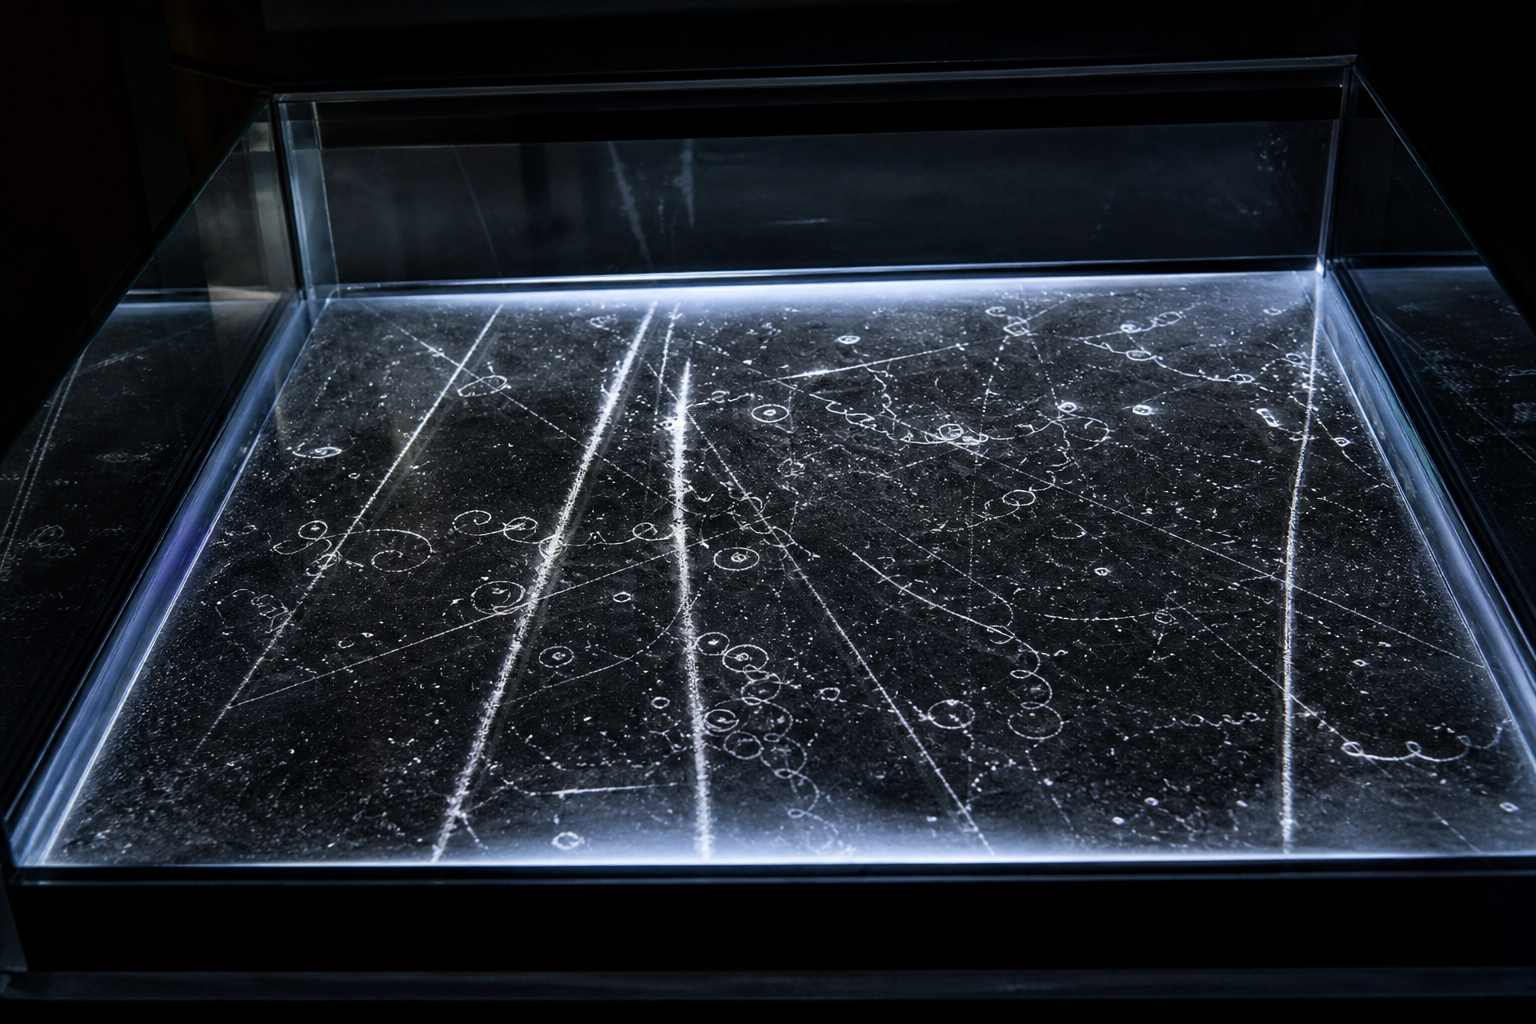
\includegraphics[width=0.58\linewidth]{images/book5/ai/b5-05-cloud-chamber.png}

{\small Partículas cargadas cruzando una cámara de niebla. Trazas como estas --- que se enroscan en los campos magnéticos y aparecen por parejas --- convirtieron $E = mc^2$ de fórmula en contabilidad cotidiana: el positrón se descubrió en una fotografía así.}
\end{omfigure}

\section{Ejercicios}

\begin{exercise}[$\star$]\label{exo:b3:relativistic-dynamics:1}
Un electrón ($mc^2 = \qty{0.511}{MeV}$) se mueve a $0.99c$. Calcúlese
$\gamma$, su momento en $\unit{MeV}/c$ y sus energías total y cinética. Las
mismas preguntas para un protón ($mc^2 = \qty{938}{MeV}$) de energía
cinética \qty{1}{GeV}.
\end{exercise}

\begin{exercise}[$\star$]\label{exo:b3:relativistic-dynamics:2}
(a) ¿Cuánta energía duerme en un gramo de materia? (b) La explosión de
Hiroshima liberó unos \qty{6e13}{J}: ¿a qué diferencia de masa equivale?
(c) El Sol radia $L = \qty{3.8e26}{W}$: ¿cuánta masa pierde por segundo, y
qué fracción de sus $\qty{2e30}{kg}$ en diez mil millones de años? (d) La
batería de su teléfono almacena \qty{5e4}{J}: ¿cuánto pesa más un teléfono
cargado?
\end{exercise}

\begin{exercise}[$\star$]\label{exo:b3:relativistic-dynamics:3}
(a) ¿Qué momento transporta por segundo el haz de un puntero láser de
\qty{5}{mW}, y qué fuerza siente el puntero? (b) ¿Qué fuerza ejerce la luz
solar (\qty{1.4}{kW/m^2}) sobre una vela solar perfectamente reflectante de
\qty{100}{m^2}? (c) Partiendo del reposo, ¿a qué velocidad se mueve una nave
vélica de \qty{10}{kg} al cabo de un mes? (d) ¿Por qué apunta la cola de
polvo de un cometa en dirección opuesta al Sol?
\end{exercise}

\begin{exercise}[$\star$]\label{exo:b3:relativistic-dynamics:4}
Práctica con unidades. (a) Muéstrese que $\unit{MeV}/c^2$ es una unidad de
masa y conviértase la masa del electrón a kilogramos. (b) ¿Cuánto es
\qty{1}{GeV/c} en $\unit{kg.m/s}$? (c) Una \omterm{def:b3:relativistic-dynamics:four-momentum}{masa invariante} al cuadrado
resulta $s = \qty{16}{GeV^2}$ (en unidades $c = 1$): ¿a qué energía del
centro de momentos corresponde? (d) ¿Por qué hacen $c = 1$ los físicos de
partículas y qué debe reinsertar un lector para obtener cifras del SI?
\end{exercise}

\begin{exercise}[$\star\star$]\label{exo:b3:relativistic-dynamics:5}
Los electrones de Bertozzi tenían energías cinéticas de $0.5$, $1$, $4.5$ y
\qty{15}{MeV}. (a) Calcúlese para cada uno la predicción de Newton
$v^2 = 2E_k/m$, en unidades de $c^2$. (b) Calcúlese el $v^2/c^2$ relativista.
(c) Su tiempo de vuelo sobre \qty{8.4}{m} a \qty{15}{MeV}: ¿qué marcó el
cronómetro y qué habría predicho Newton? (d) La energía de los electrones se
midió además calorimétricamente --- por su calor al impactar ---: ¿por qué
era ese paso el verdadero núcleo del experimento?
\end{exercise}

\begin{exercise}[$\star\star$]\label{exo:b3:relativistic-dynamics:6}
El pion cargado se desintegra en reposo: $\pi^+ \to \mu^+\nu$, $m_\pi c^2 =
\qty{139.6}{MeV}$, $m_\mu c^2 = \qty{105.7}{MeV}$, $m_\nu \approx 0$.
(a) Muéstrese que $pc = (m_\pi^2 - m_\mu^2)c^4/2m_\pi c^2$ y evalúese.
(b) La energía cinética y la velocidad del muon. (c) La energía del
neutrino. (d) En vuelo con $\gamma_\pi = 50$, ¿cuáles son las energías
máxima y mínima del muon en el laboratorio (desintegración hacia delante y
hacia atrás)?
\end{exercise}

\begin{exercise}[$\star\star$]\label{exo:b3:relativistic-dynamics:7}
La \omterm{def:b3:relativistic-dynamics:four-momentum}{masa invariante} en acción. (a) Dos fotones de \qty{200}{MeV} cada uno
vuelan formando $60^\circ$ entre sí: calcúlese la \omterm{def:b3:relativistic-dynamics:four-momentum}{masa invariante} de la
pareja. (b) Un pion neutro ($m_{\pi^0}c^2 = \qty{135}{MeV}$) se desintegra
en dos fotones: ¿cuál es la \omterm{def:b3:relativistic-dynamics:four-momentum}{masa invariante} de la pareja de fotones, en
cualquier sistema? (c) Explíquese cómo un experimento ``descubre'' una
partícula como una joroba en la distribución de \omterm{def:b3:relativistic-dynamics:four-momentum}{masa invariante} de sus
productos de desintegración. (d) Dos fotones de igual energía vuelan
exactamente paralelos: ¿\omterm{def:b3:relativistic-dynamics:four-momentum}{masa invariante}? ¿Qué dice esto sobre el sistema
propio de un haz de luz?
\end{exercise}

\begin{exercise}[$\star\star$]\label{exo:b3:relativistic-dynamics:8}
Contabilidad del LHC (protones de $E = \qty{6.8}{TeV}$). (a) $\gamma$ y el
déficit de velocidad $c - v$ (úsese $c - v \approx c/2\gamma^2$). (b) La
frecuencia de revolución en el anillo de \qty{27}{km} y el número de vueltas
por segundo. (c) La energía almacenada en un haz de \num{3e14} protones, en
kilogramos de TNT (\qty{4.2e6}{J/kg}). (d) El equivalente en masa de la
energía cinética de los dos haces, en microgramos --- materia a punto de
fabricarse.
\end{exercise}

\begin{exercise}[$\star\star$]\label{exo:b3:relativistic-dynamics:9}
Fotones que chocan. (a) Muéstrese que un solo fotón en el vacío no puede
desintegrarse en un par electrón--positrón, por energético que sea (úsese el
invariante). (b) Frente a un segundo fotón de energía $\epsilon$ y
frontalmente, muéstrese que la creación de pares exige
$E\epsilon \ge (m_{\text{e}}c^2)^2$. (c) ¿Qué compañero necesita un fotón de
\qty{511}{keV}? ¿Y un rayo X de \qty{50}{keV}? (d) El universo está lleno de
luz estelar y del fondo cósmico de microondas: ¿qué predice (b) para el
alcance de los rayos $\gamma$ de TeV a través del espacio intergaláctico?
\end{exercise}

\begin{exercise}[$\star\star\star$]\label{exo:b3:relativistic-dynamics:10}
Compton, con \omterm{def:b3:relativistic-dynamics:four-momentum}{cuadrimomentos}. Un fotón de longitud de onda $\lambda$ golpea
un electrón en reposo y se dispersa con ángulo $\theta$. (a) Escríbase la
conservación del \omterm{def:b3:relativistic-dynamics:four-momentum}{cuadrimomento} y despéjese el invariante del electrón final.
(b) Dedúzcase
\[
\lambda' - \lambda = \frac{h}{m_{\text{e}}c}\,(1 - \cos\theta) .
\]
(c) Evalúense $h/m_{\text{e}}c$ y el desplazamiento máximo; ¿por qué es el
efecto invisible con luz visible y decisivo para los rayos X? (d) ¿Qué
estableció la medida de Compton de 1923 sobre la luz que el efecto
fotoeléctrico no había establecido?
\end{exercise}

\begin{exercise}[$\star\star\star$]\label{exo:b3:relativistic-dynamics:11}
El final del espectro de rayos cósmicos. El universo está bañado en fotones
de microondas de energía típica $\epsilon = \qty{6e-4}{eV}$. Un protón de
energía $E$ que golpea uno frontalmente puede excitarse hasta la resonancia
$\Delta$ ($m_\Delta c^2 = \qty{1232}{MeV}$) y pierde energía cada
vez. (a) Muéstrese que la condición de umbral es aproximadamente $4E\epsilon =
(m_\Delta^2 - m_{\text{p}}^2)c^4$. (b) Calcúlese el $E$ umbral.
(c) Por encima de él, el universo es opaco a los protones más allá de unos
\qty{100}{Mly}: ¿qué predice esto para el espectro observado de rayos
cósmicos (el corte de Greisen--Zatsepin--Kuzmin)? (d) Se han registrado
rayos cósmicos de $\qty{3e20}{eV}$ --- las partículas ``Oh-My-God'': ¿qué
exige su existencia de sus fuentes?
\end{exercise}

\begin{exercise}[$\star\star\star$]\label{exo:b3:relativistic-dynamics:12}
El cohete de fotones. Un cohete de masa inicial $m_{\text{i}}$ emite su
escape como un haz de luz colimado y alcanza la velocidad $\beta c$. (a)
Conservando energía y momento entre el principio y el final, muéstrese que
\[
\frac{m_{\text{i}}}{m_{\text{f}}} =
\sqrt{\frac{1 + \beta}{1 - \beta}} = \eu^{\varphi} ,
\]
la exponencial de la rapidez --- la ecuación relativista de Tsiolkovski con
el mejor escape posible. (b) ¿Razón de masas para alcanzar
$0.9c$? ¿Y para alcanzar $0.9c$ y \emph{detenerse} en el destino? (c) El
haz hay que fabricarlo de algún modo: con aniquilación materia--antimateria
de eficiencia perfecta, ¿cuántos kilogramos de antimateria por kilogramo de
carga útil para el viaje de ida a $0.9c$? (d) La producción mundial de
antiprotones es de nanogramos al año: conclúyase, en una frase, sobre los
cohetes de fotones.
\end{exercise}

\begin{omfigure}
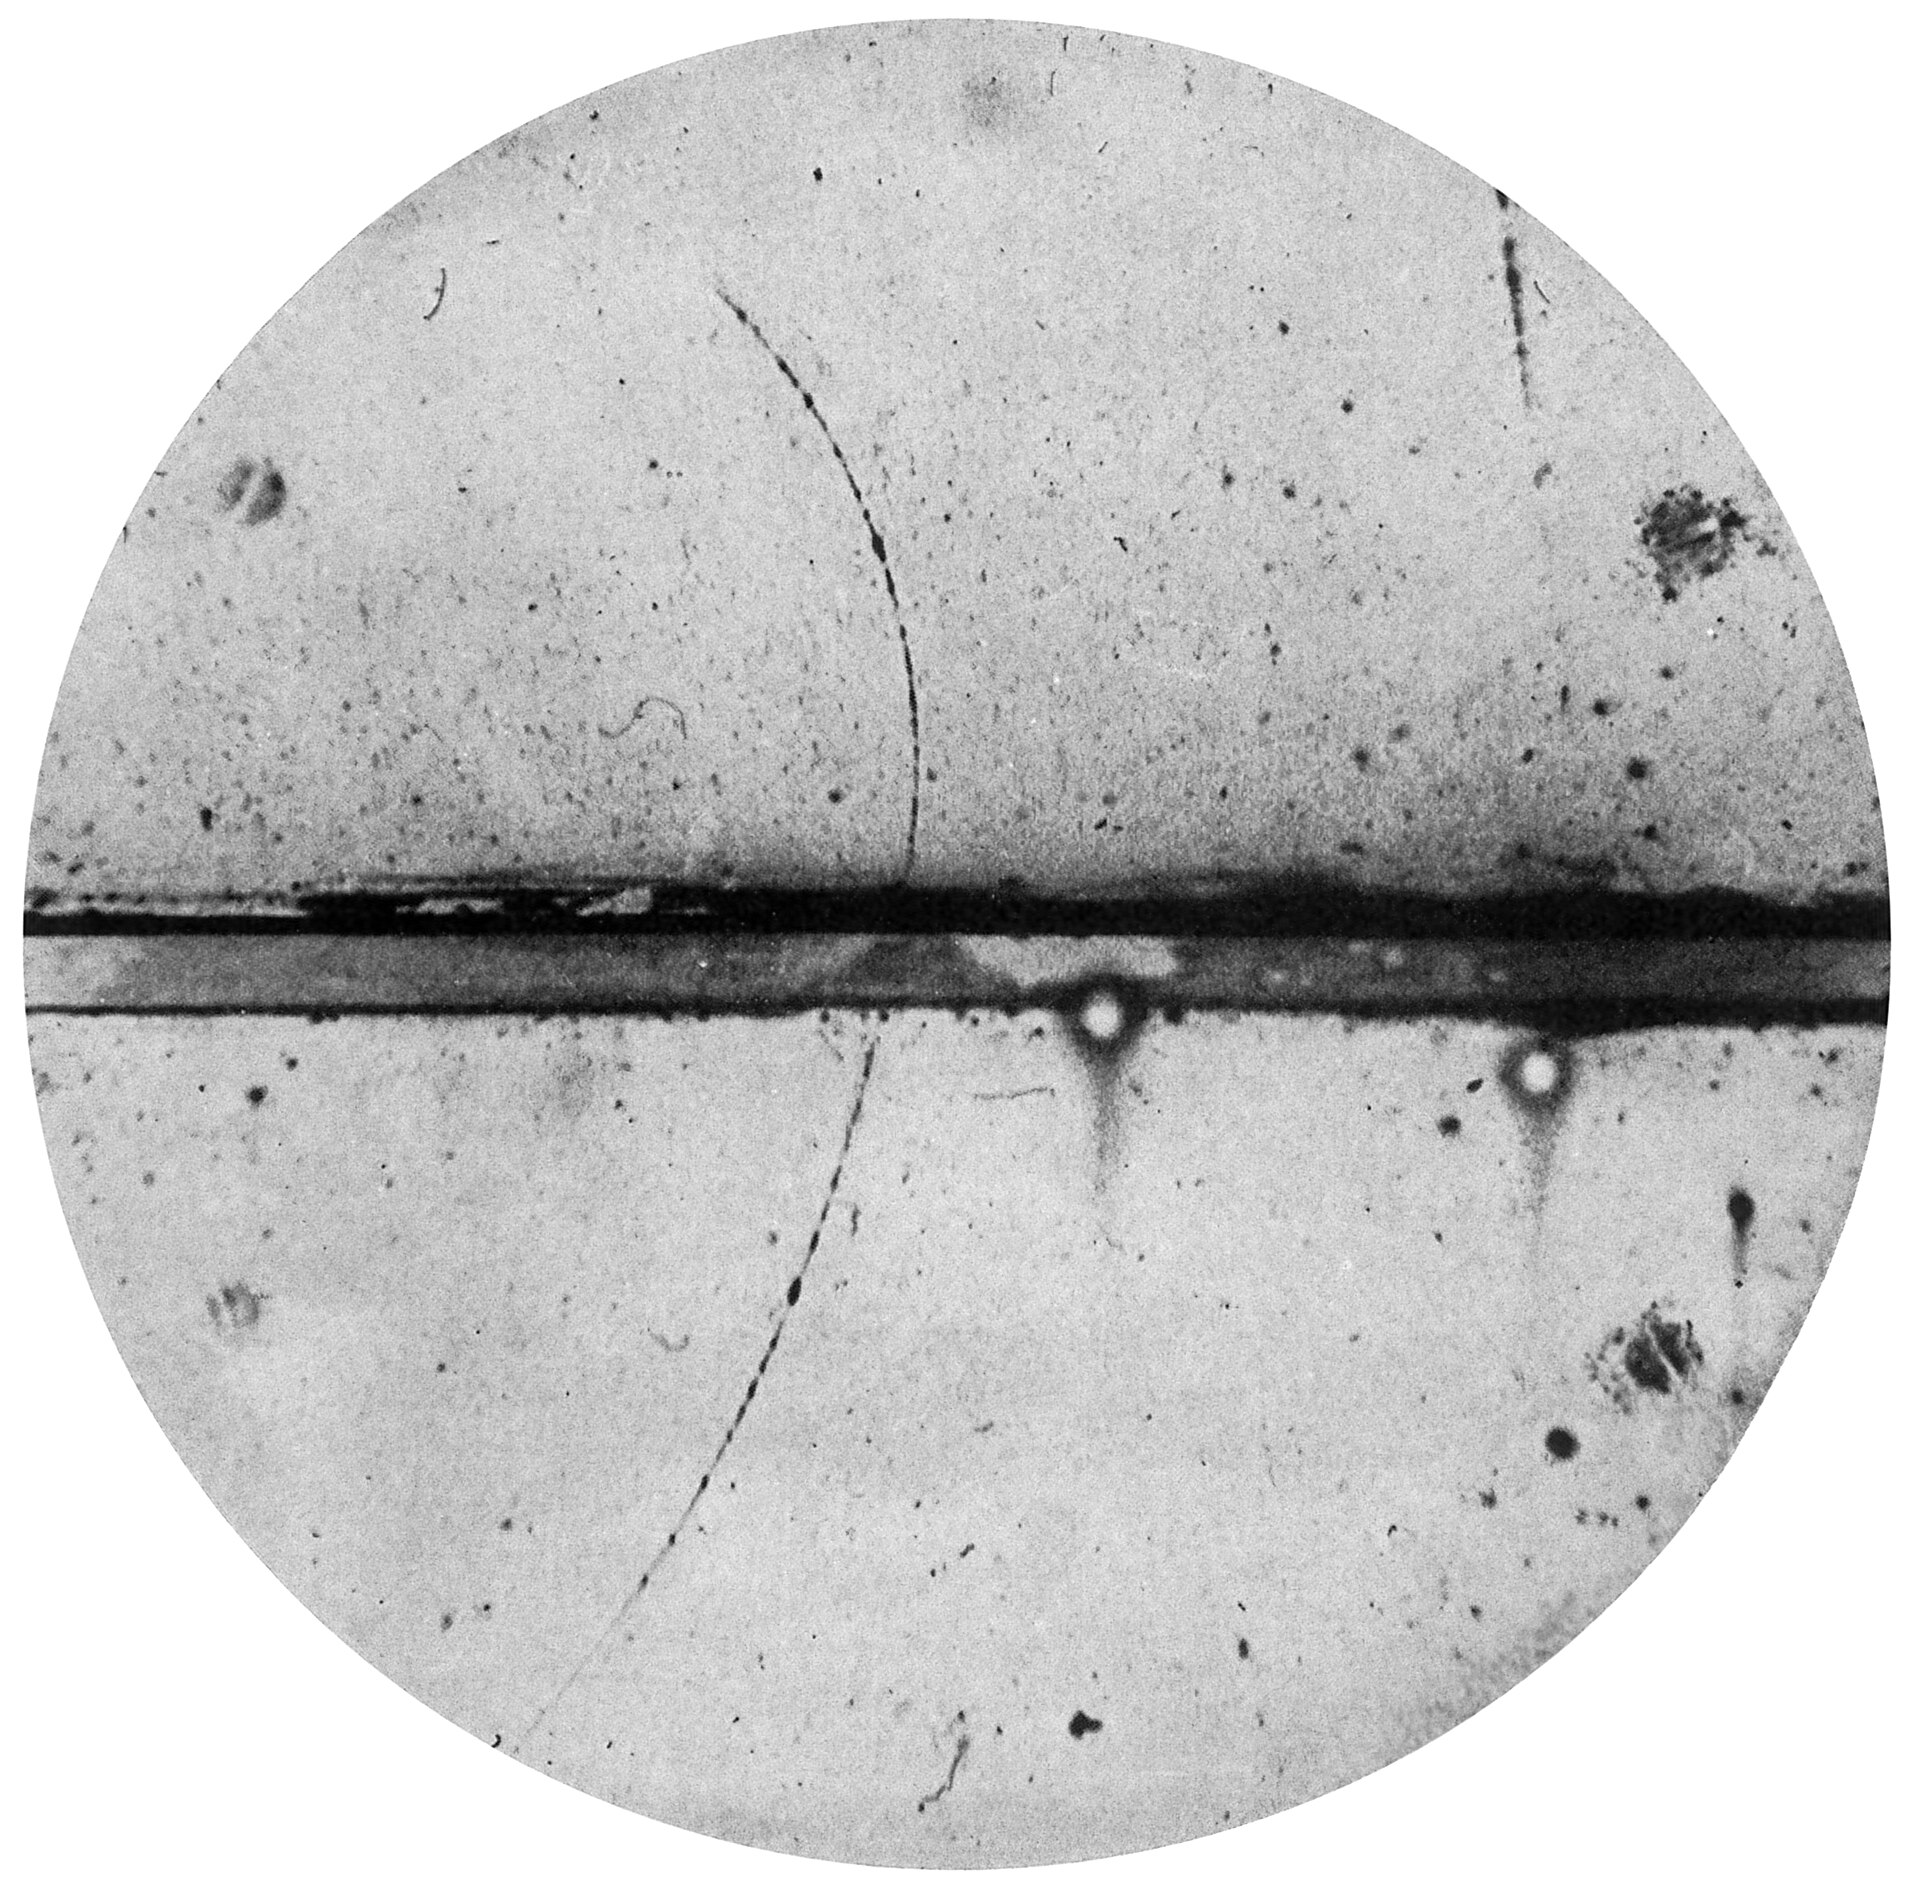
\includegraphics[width=0.5\linewidth]{images/book5/photo-positron-anderson.jpg}

{\small El descubrimiento de la antimateria (Carl D. Anderson, 1932, dominio público): un único positrón que asciende atravesando la placa de plomo de la cámara de niebla, curvándose al revés que un electrón y demasiado cerrado para ser un protón --- la contabilidad de $E = mc^2$ sorprendida marchando al revés.}
\end{omfigure}

\section{Problema: fabricar materia --- el antiprotón y el Bevatrón}

\begin{problem}[{Problema de fin de semana --- cómo puso precio al
antimundo la conservación del momento}]\label{pb:b3:relativistic-dynamics:1}
Las ecuaciones de Dirac exigían, desde 1931, que el protón tuviese un
gemelo especular de carga opuesta. Fabricar uno significaba comprar su
\omterm{def:b3:relativistic-dynamics:momentum-energy}{energía en reposo} con energía del haz --- y la conservación del momento fijó
el precio. Este problema lo tasa, diseña la máquina que lo pagó y sigue el
descubrimiento de 1955. Datos: $m_{\text{p}}c^2 = \qty{938.3}{MeV}$; la
carga y el \emph{número bariónico} (protones y neutrones $+1$, antiprotones
$-1$) se conservan en toda reacción.

\medskip\noindent\textbf{Parte I --- La caja de herramientas del \omterm{def:b3:relativistic-dynamics:four-momentum}{cuadrimomento}.}
\begin{enumerate}
  \item Para una partícula, muéstrese $E^2 - p^2c^2 = m^2c^4$ a partir de
        las definiciones de $E$ y $\vect p$.
  \item Para un sistema, ¿por qué es $E_{\text{tot}}^2 -
        p_{\text{tot}}^2c^2$ el mismo en todos los sistemas y a qué
        equivale en el sistema del centro de momentos?
  \item Un haz de protones de energía $E$ golpea un protón en reposo:
        muéstrese que $M^2c^4 = 2m_{\text{p}}^2c^4 + 2E\,m_{\text{p}}c^2$.
  \item Compruébense los dos límites: a baja energía, $Mc^2 \to
        2m_{\text{p}}c^2$; a alta energía, $Mc^2 \approx
        \sqrt{2E\,m_{\text{p}}c^2}$ --- la ley de la raíz cuadrada.
  \item Una reacción solo está permitida si $Mc^2$ alcanza la suma de las
        masas en reposo de los productos, con todos ellos en reposo en el
        sistema del centro de momentos en el umbral: justifíquese esta
        última cláusula.
  \item ¿Por qué no puede recuperarse jamás la energía cinética de los
        productos en el laboratorio para crear partículas sobre un blanco
        fijo?
\end{enumerate}

\medskip\noindent\textbf{Parte II --- El precio del antiprotón.}
\begin{enumerate}[resume]
  \item En las colisiones $p + p$, la reacción más barata que fabrica un
        antiprotón $\bar p$ debe fabricar además un protón \emph{de más}:
        escríbase y justifíquese con la carga y el número bariónico.
  \item Muéstrese que el umbral exige $Mc^2 = 4m_{\text{p}}c^2$.
  \item Dedúzcase la energía de haz necesaria $E = 7m_{\text{p}}c^2$ y la
        energía cinética $T = 6m_{\text{p}}c^2$; evalúese $T$.
  \item En el umbral, ¿qué fracción de la energía cinética del haz se
        convirtió realmente en masa en reposo nueva (los
        $2m_{\text{p}}c^2$ correspondientes)? ¿Dónde está el resto?
  \item En un colisionador frontal $p$--$p$, ¿qué energía cinética
        \emph{por haz} necesitaría la misma reacción? Compárense los dos
        diseños.
  \item En 1954 no existía ningún colisionador (los haces eran demasiado
        tenues para acertarse entre sí): ¿qué hecho práctico obligó a
        elegir el blanco fijo y qué costó eso en energía de haz?
\end{enumerate}

\medskip\noindent\textbf{Parte III --- Diseñar el Bevatrón.}
La máquina construida en Berkeley alcanzó $T = \qty{6.2}{GeV}$ ---
holgadamente por encima del umbral --- con campos dipolares de $B =
\qty{1.56}{T}$.
\begin{enumerate}[resume]
  \item Calcúlense la energía total y el momento del haz a máxima energía.
  \item Calcúlese el radio de curvatura $r = p/qB$ y compárese con los
        \qty{15.2}{m} de la máquina.
  \item Calcúlense la velocidad del protón y la frecuencia de revolución en
        el anillo de longitud $2\pi r$.
  \item En la inyección, los protones llegan con \qty{10}{MeV} de energía
        cinética: calcúlese su velocidad y explíquese por qué la frecuencia
        aceleradora debía \emph{barrer} durante cada ciclo (¿qué dos
        magnitudes cambian al crecer $E$?).
  \item Con unos \qty{1.5}{kV} ganados por vuelta, ¿cuántas vueltas y
        cuánto tiempo dura un ciclo de aceleración?
  \item El nombre ``Bevatrón'' venía de BeV, miles de millones de
        electronvoltios: enúnciese en una línea qué física fijó la cifra de
        diseño de $6$ y pico BeV.
\end{enumerate}

\medskip\noindent\textbf{Parte IV --- El descubrimiento, 1955.}
\begin{enumerate}[resume]
  \item Un imán curva a cada candidato sobre una circunferencia: explíquese
        por qué eso selecciona partículas por \emph{momento} ($r = p/qB$)
        y no por energía ni por velocidad --- y por qué un haz
        seleccionado en momento mezcla todavía especies distintas.
  \item El haz sobre un blanco de cobre producía torrentes de piones
        negativos ($m_\pi c^2 = \qty{139.6}{MeV}$) entre los que se
        escondían unos pocos antiprotones. El espectrómetro seleccionaba
        negativos de momento $p = \qty{1.19}{GeV}/c$: calcúlense la velocidad
        de un antiprotón y la de un pion con ese momento.
  \item A lo largo de los \qty{12}{m} de vuelo, calcúlense los dos tiempos de
        recorrido: ¿qué resolución temporal necesitó el descubrimiento?
  \item Una segunda firma independiente empleaba contadores de Cherenkov,
        que solo se disparan por encima de un umbral de velocidad: ¿qué
        partícula se dispuso que los disparase y por qué importa la
        redundancia en un descubrimiento?
  \item Chamberlain y Segrè contaron alrededor de un antiprotón por cada
        $\num{44000}$ piones: ¿por qué garantizaba el argumento del umbral
        que el ritmo sería diminuto incluso por encima de él?
  \item Un antiprotón acaba encontrándose con un protón y se aniquila:
        ¿cuánta energía se libera por suceso y en qué, típicamente?
  \item Resúmase el resultado con nombre propio: la conservación del
        \omterm{def:b3:relativistic-dynamics:four-momentum}{cuadrimomento} tasó el antiprotón en $T = 6m_{\text{p}}c^2 =
        \qty{5.6}{GeV}$ sobre un blanco fijo; un sincrotrón de
        \qty{6.2}{GeV} y \qty{15}{m} lo pagó, y el antimundo se convirtió
        en un hecho de laboratorio --- el Premio Nobel de 1959.
\end{enumerate}
\end{problem}
